
\subsection{System Model}
\begin{figure}
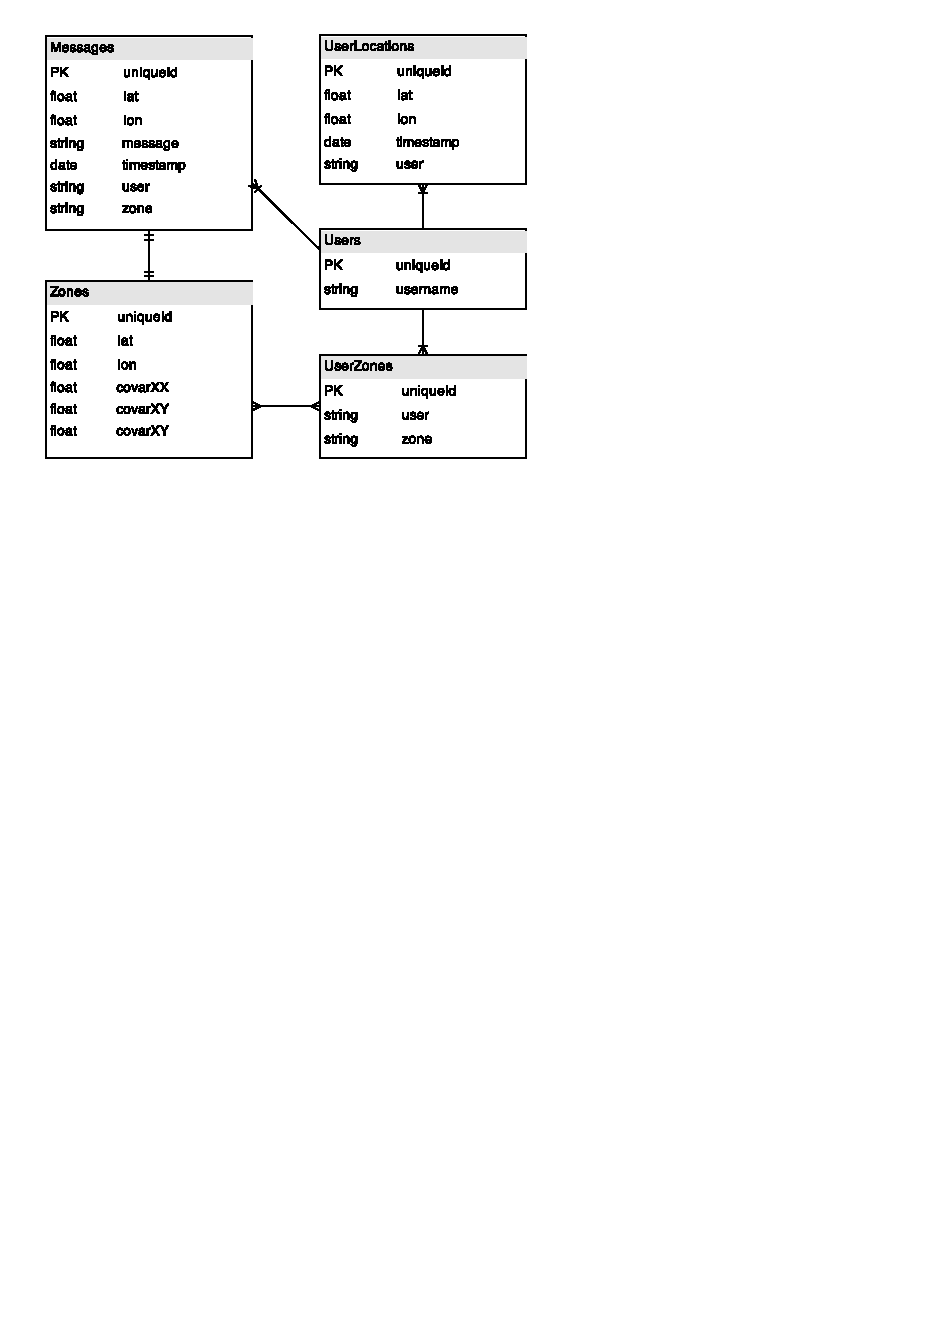
\includegraphics{figs/systemModel}
\caption{GeoChat Database structure.  The user pings the server regularly with their location which is used to determine which zones they should be a part of, and which messages they can see.  Zones behave much like geo-spatial conversation threads, where all messages are public within them.  Zone covariance defines the size and shape of the zones.}
\label{systemModel}
\end{figure}

Our system was implemented with a relatively simple database model shown in figure~\ref{systemModel}.  Firebase allows developers to watch one key on a table for instantaneous updates, and for this reason it is critical to ensure that we can indicate whether a message will be relevant to a user with a single key.  To this end we reorganized our code so that instead of watching a pair of lat/long co-ordinates we instead watch a particular zone.  The zones are calculated by expectation maximization of a gaussian mixture model, discussed in the implementation section.

\subsection{Problem Statement}
Terms, definitions, components
